\chapter{Overview}
\label{chp:overview}
\ProductName{} can run on a single Unix host or several co-operating machines.
The central white area of the block diagram shows the possible components of \ProductName{} on a Unix machine. The shaded area indicates the
entities, outside of that machine's \ProductName{} system boundary, which use or provide services to it.

 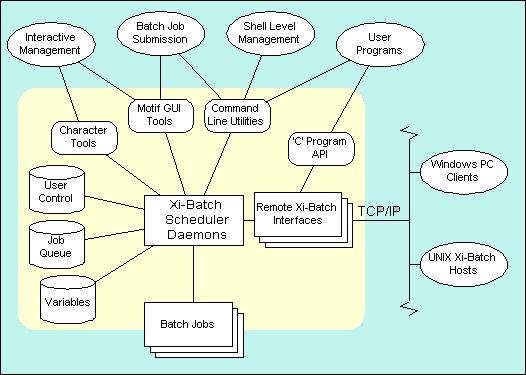
\includegraphics[width=13.771cm,height=9.922cm]{img/ref1.jpg} 

At the heart of \ProductName{} is the scheduler daemon \progname{btsched}. This daemon manages the batch jobs and
the job control variables, which are used for handling dependencies. There are two instances of \progname{btsched} running on a
stand alone system, or three if co-operating with other \ProductName{} hosts. Co-operating \ProductName{} hosts require connection via a network that
provides TCP/IP services.

\progname{btsched} maintains the job and variable shared memory segments, writing them out to file when changes are made. It
forks to provide one process to monitor running processes and one to accept messages on the message queue. It forks again to provide the
third \progname{btsched} to handle the network interface if this mode of operation is used.

When an interactive queue management tool (e.g. \PrBtq{} or \PrXmbtq{}) process is
started, it arranges with \progname{btsched} to be sent signals to advise it of changes in the job queue or variable list.

All requests, by \PrBtq{} and other processes, are dealt with by sending a message on the message queue and receiving
replies on the same message queue.

\section{IPC used by \manualProduct{}}

\ProductName{} uses one message queue to communicate with the scheduler process, \progname{btsched}. Two shared memory segments are
used to hold records of jobs and variables. These records are periodically written out to the files
\filename{btsched\_jfile} and \filename{btsched\_vfile} respectively in the spool directory, by default \spooldir.
A further shared memory segment is used as buffer space for passing job details, as the size of messages which may be sent on message queues is limited on many systems. One group of semaphores controls access to the shared memory segments, and another group is used for network locking.

The IPC facilities can be recognised by running \progname{ipcs}. The items in question are owned by \batchuser{} with a key of \filename{0x5869Bxxx}.

\section{Directory and File Structure}
The files which comprise \ProductName{} are held in various directories depending upon their nature. With the exception of global configuration
files the installation can be tailored to suit local practices and
standards.

\begin{itemize}
\item Global configuration files are always held in the \filename{\etcname} directory.
\item User programs can be placed in any directory which is on the \ProductName{} users' \filename{PATH}.
\item Internal programs and data are held in two or sometimes three separate directories.
\item There are some other useful programs, such as \PrXbRipc{}, \PrXbCjlist{} etc, which are also placed in the user path directory.
\end{itemize}

If your public program directory is \filename{/usr/lbin} (some machines use \filename{/usr/local/bin}) and the spool
directory is under \filename{/usr} (some are under \filename{/var}), then the default installation will look like
this:

 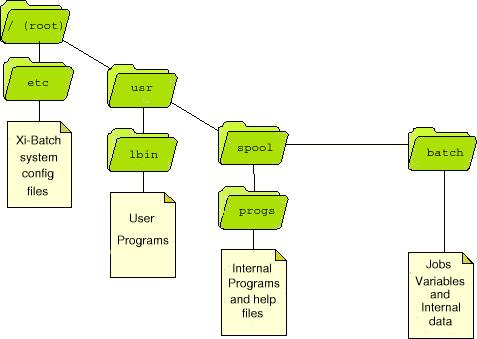
\includegraphics[width=16.953cm,height=11.441cm]{img/ref2.jpg} 

\subsection{Internal Directories}
\ProductName{} uses three logical directories to hold the internal programs and data. These are usually mapped onto two physical directories. A
default installation would look like this:


\begin{figure}
\centering
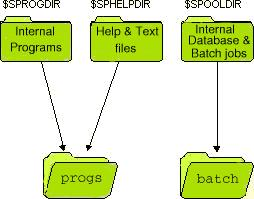
\includegraphics[width=13.808cm,height=9.065cm]{img/ref3.jpg}
\end{figure}

These directories may be relocated by assignment to the three environment variables: \filename{SPROGDIR},
\filename{SPHELPDIR} and \filename{SPOOLDIR}. These environment variable assignments may be placed in the master
configuration file, \masterconfig, to ensure consistency. The default directories are as follows:

\begin{center}
\begin{tabular}{|l|l|l|}\hline
\bfseries Default location & \bfseries Environment variable & \bfseries Function\\\hline
\spooldir & \filename{SPOOLDIR} & Jobs and other internal data.\\
\progsdir & \filename{SPROGDIR} & Internal programs\\
\helpdir & \filename{SPHELPDIR} & Global help and message files\\\hline
\end{tabular}
\end{center}

Take care not to assign values to these environment variables arbitrarily; very strange things will happen if one part of \ProductName{} is
using one set of directories and some other part is using another!

\subsection{Internal Programs}
These include the scheduler, network connection daemon, \progname{xbnetserv} and the utilities used by them. They
are held in the internal programs directory. With certain exceptions it is not intended that users should ever invoke these programs.

The file structure of the internal programs is flat within their directory.

\subsection{Batch directory files}
The following \ProductName{} internal files are held in the spool directory, which by default is \spooldir:

\begin{center}
\begin{tabular}{|l|l|}\hline
\bfseries File &
\bfseries Purpose\\\hline
\filename{btufile\IfXi{6}IfGNU{1}} & User permissions\\
\filename{btcharges\IfXi{6}IfGNU{1}} & User charges (now deprecated)\\
\filename{cifile} & Specification of command interpreters\\
\filename{holfile} & Days set to be holidays\\
\filename{btsched\_jfile} & Saved record of jobs\\
\filename{btsched\_vfile} & Saved record of variables\\
\filename{btsched\_reps} & Report file holding any messages output by \progname{btsched}\\
\filename{pwdump\IfXi{6}IfGNU{1}} & Optional saved password map file (now deprecated)\\
\filename{SPnnnnnnnn} & Queued jobs\\
\filename{SOnnnnnnnn} & Standard output of pending jobs\\
\filename{ERnnnnnnnn} & Standard error of pending jobs\\
\filename{NTnnnnnnnn} & Local copy of remote job\\\hline
\end{tabular}
\end{center}

The above files are owned by \batchuser{}. Unused copies of the last four kinds of files may safely be deleted. The
\genericargs{nnnnnnnn} component of the file name is derived from the batch job number.

\subsection{Help and Message files}
\IfXi{In common with other Xi Software products, }\ProductName{} reads all of its
messages from a series of text files (Apart from the ``help I cannot find the message file'' messages).
The user may adjust these to tailor the command interface, help and error messages to be suitable for the particular installation.
These are \textit{system-wide} message files. It is also possible to set up customised versions for individual users or applications.

The following files are, by default, owned by \batchuser{} and held in the directory, by default \helpdir.

\begin{center}
\begin{tabular}{|l|l|}\hline
\bfseries File &
\bfseries Purpose\\\hline
\filename{btq.help} & Screen layout, messages and key assignments for \PrBtq{}\\
\filename{btuser.help} & Screen layout, messages and key assignments for \PrBtuser{}\\
\filename{btrest.help} & Messages and arguments for other user programs\\
\filename{btint-config} & Message file for \progname{btsched}, \progname{btwrite} and \progname{xbnetserv}\\
\filename{filemon.help} & Message file for file monitor option, \PrBtfilemon{}.\\
\filename{xmbtq.help} & Message file for \PrXmbtq{}\\
\filename{xmbtr.help} & Message file for \PrXmbtr{}\\
\filename{xmbtuser.help} & Message file for \PrXmbtuser{}\\\hline
\end{tabular}
\end{center}
Please refer to the chapters on Configuration and Extending the toolset for details of how to modify these files.

\subsection{Configuration files held in \etcname}
\ProductName{} uses up to three files held in the system directory \filename{\etcname}.

\subsubsection{\manualProduct{} Hosts File}
The file \hostsfile{} is used on networked installations of \ProductName{} to denote details of the remote hosts and clients to which
connection is to be made.

Each line in the file other than blank lines or comment lines (introduced with a \# sign) consists of up to 4 fields. These are as
follows:

\begin{enumerate}
\item The \textit{hostname} to attach to or an internet address such as \filename{197.3.9.1}.
For DHCP clients, this gives the Windows user name to be recognised (case insensitive).
\item An \textit{alias name} by which the remote host is to be referred to within \ProductName{}.
The user can give either the host name or the alias name in commands such as \PrBtconn{} but displays (as in \PrBtq{} or \PrBtvlist{}) will
always use the alias. For DHCP clients, this gives the Unix user name (if different) corresponding to the given Windows user name.

An alias or Unix user name can be omitted by just putting a single ``\exampletext{{}-}'' sign.

An alias \textit{must} be supplied if the host name is given as an internet address.
\item \textit{Flags}, which are further described below.
\item A numeric time-out value in seconds. The default if this is omitted is 1000. This is most important for Windows clients, as it also
denotes a time after which the connection becomes ``stale'' and must be refreshed, possibly by re-entering the password.
\end{enumerate}
The flags field is one or more of the following separated by commas.

\begin{tabular}{|l | p{12cm}|}
\hline
\filename{probe} &
Denotes that the scheduler should check that the specified host is active before attempting a connection.\\\hline
\filename{manual} & Denotes that no connection is attempted until the operator
invokes one with \PrBtconn{}.\\\hline
\filename{external} & Denotes that the named host is some external system. Currently
this has no meaning in \ProductName{}.\\\hline
\filename{dos(user)} & For a Microsoft Windows client PC. Requests are allocated by default to the username given.\\\hline
\filename{client(user)} & Is a synonym for \filename{dos(user)}.\\\hline
\filename{clientuser} & Denotes that the first and second fields are
\genericargs{user}, not machine names, for DHCP clients.
As a special case, if the first field is default and the second field
is a user name on the Unix host, then a default user name is thereby
supplied for all unknown Windows users.\\\hline
\filename{clientuser(machine)} & As \exampletext{clientuser}, but denotes that the default client machine is given, otherwise a password is
required.\\\hline
\filename{trusted} & Exchange information with this Unix host about Windows client users. (This is now deprecated.)\\\hline
\filename{pwchk} & Demand Unix password from Windows clients in all cases.\\\hline
\end{tabular}

For example:

\begin{expara}

mach19 \ \ \ \ \ \ \ \ red \ \ \ probe

mach20 \ \ \ \ \ \ \ \ green \ probe,manual

192.112.238.7 \ yellow probe

WS21 \ \ \ \ \ \ \ \ \ \ blue \ \ dos(jmc) \ \ \ \ \ \ \ \ 30

john \ \ \ \ \ \ \ \ \ \ jmc \ \ \ clientuser,pwchk

default \ \ \ \ \ \ \ guest \ clientuser

\end{expara}

This provides for 4 machines, where host names are \exampletext{mach19}, \exampletext{mach20}, \exampletext{WS21}
an IP address and also a user name for DHCP clients. These are given aliases of \exampletext{red}, \exampletext{green}, \exampletext{yellow} and
\exampletext{blue}.

In the first and third case any connection will be tested first before continuing.

In the \exampletext{green} case no connection is attempted until the user types,

\begin{expara}

\BtconnName{} green

\end{expara}

or

\begin{expara}

\BtconnName{} mach20

\end{expara}

The \exampletext{blue} machine is a Microsoft Windows workstation. Requests will be assumed to come from user
\exampletext{jmc}. Time-outs of 30 seconds apply to requests.

Next the Windows user name of \exampletext{john} on any Windows PC is translated to a Unix user name of \exampletext{jmc},
after checking the password.

Finally, any unrecognised Windows user name is treated as the Unix user name of guest.

The utility program \PrHostedit{} (or the GTK+ version \progname{xhostedit}) may be used to create or edit this
file with appropriate checks.

Note that the mapping of UNIX names to Windows names in this file is deprecated -- this is now done in the user mapping file.

\paragraph{Multiple IP addresses}
It is sometimes unclear what the local address is, i.e. the IP address corresponding to the host on which it is running. It is important for
the software to know this, as other hosts will use this to identify jobs and variables belonging to the host. It is possible to specify
this in the hosts file thus:

\begin{expara}

localaddress 193.112.238.250

\end{expara}

The \exampletext{localaddress} statement must be the first item (other than comments or blank lines) in the host file. The address
given can be either a host name or an IP address.

The address can also be obtained each time it is started by connecting to another host and running \filename{getsockname()} on the
result. To signify this, the following format is used.

\begin{expara}

Localaddress GSN(www.google.com,80)

\end{expara}

The integer gives a port number to use.

The host name can be given as above, or an IP address can be used.

\subsubsection{\manualProduct{} Master Configuration File}
In order to work properly, the scheduler process and all the other programs must be started with the same environment variables. For
convenience, the environment may be initialised for each program by creating a master configuration file \masterconfig.

This file contains a list of environment variable assignments. Any environment variables not defined on entry to any of the programs are
initialised from this file. Any environment variables used by \ProductName{} may be included in this file, not just those shown in the example.

For example:

\begin{expara}

SPOOLDIR:/usr1/spool/batch

SPROGDIR:/usr1/spool/bin

MAILER=/usr/lib/sendmail

\end{expara}

An environment variable declared using the equality sign \exampletext{=} will be included in the environment of all
batch jobs that are submitted. This may not be wanted for all variables, in particular the scheduler directories pointed to by
\filename{SPOOLDIR}, \filename{SPROGDIR} and \filename{SPHELPDIR}. To avoid jobs inheriting environment
variables from the configuration file declare them using the colon, \exampletext{:} , instead of the equals sign,
\exampletext{=}.

Please note that the text to the right of the colon or \exampletext{=} sign is taken literally; there is no recursive
expansion of \exampletext{\$name} constructs except for the message file names \filename{BTQCONF},
\filename{BTUSERCONF} and \filename{BTRESTCONF} (where it is limited to 10 recursive expansions).

\subsubsection{User Mapping file}
The user map file provides a mapping between external names, usually Windows user names, and UNIX names.

The file is in \usermap, and consists (apart from comments introduced by the \filename{\#} character) of
lines of the format

\begin{expara}

unix-user:windows-user

\end{expara}

For example:

\begin{expara}

\# User mapping file

jmc:john collins

sec:sue collins

guest:default

\end{expara}

The final entry gives a default user if a named user is not found in the file.

UNIX users not found on the host are silently ignored.

\subsubsection{\manualProduct{} Static Environment File}
To avoid every job having to have all the environment variables in it, thus saving space, the static environment file,
\batchenv{}, is provided. The commands that submit jobs will only store ``differences'' from this file in each job.
This is provided to avoid saving large amounts of environment information with each job.

Alternative files to \batchenv{} can be specified by including the following line in \linebreak[20]\masterconfig:

\begin{expara}

BATCHENV:file1,file2....

\end{expara}

These files are read in sequence and constitute the new environment.

\section{Job and Variable Modes}
Each job and variable is given a \textit{protection mode}. This consists of a set of permissions dictating how various users may, or may not,
access the job or variable. The modes are like those on Unix files, providing \textit{user}, \textit{group} and \textit{other} access. An
expanded set of permissions has been devised to enable the permissions to control separate operations.

The permissions are as follows, one set for each of \textit{user}, \textit{group} and \textit{others}:

\begin{center}
\begin{tabular}{|l l|}
\hline
\bfseries Permission &
\bfseries Function\\\hline
Read & Job or variable may be read\\
Write & Job or variable may be written\\
Reveal & Job or variable is `visible' to user\\
Read modes & Modes may be displayed\\
Set modes & Modes may be set\\
Give away Owner & Ownership may be given away\\
Give away Group & Group may be given away\\
Assume Ownership & Ownership may be assumed\\
Assume Group & Group may be assumed\\
Delete & Job or variable may be deleted\\
Kill (jobs only) & Job may be killed\\\hline
\end{tabular}
\end{center}
Only the primary group of a user is considered when evaluating group access permissions.

The visibility of variables and jobs can be set to the local machine only or all networked \ProductName{} machines.

\subsection{Change of owner and group}
Changes of owner and group take place in 2 stages for security.

\begin{enumerate}
\item The existing owner, or someone with \textit{give away} permission gives the job or variable away to a designated owner or group. This
designated owner or group is noted, but the change has no effect at this stage.
\item The designated owner or a user with that group will have to explicitly \textit{assume ownership} of the job or variable. This owner
or group must also have the appropriate permission.
\end{enumerate}

This 2-stage process is to prevent the security violations of unauthorised assumption of ownership, and also to prevent jobs from
being run masquerading as unauthorised users.

A user with \textit{write administration file} privilege does not have to go through this procedure. Changes to owner or group of a job or
variable by such users are immediate and complete.

\subsection{Initialisation of modes}
The modes of jobs and variables are set when they are created, however users authorised by the mode may reset them subsequently.

In the case of \textit{jobs}, the modes set by the option \exampletext{{}-M} to \PrBtr{} are used, in
default of which a set of default modes for the given user are set.

In the case of \textit{variables}, the mode is set from the default modes for the given user.

A user may be permitted to reset his own default modes with the \textit{change default modes} privilege as described in a later
chapter, using \PrBtuser{}. A system-wide `default default mode' is given to each new user, along with a default set of privileges.

As distributed, \ProductName{} will assign the following default modes to jobs and variables:
\label{overview:defmodes}
\begin{center}
\begin{tabular}{|lllllll|}\hline
& & \bfseries Jobs& & & \bfseries Variables & \\
&\bfseries User & \bfseries Group & \bfseries Other & \bfseries User & \bfseries Group & \bfseries Other\\\hline
Read & Yes & Yes & No & Yes & Yes & No\\
Write & Yes & No & No & Yes & No & No\\
Reveal & Yes & Yes & Yes & Yes & Yes & Yes\\
Read Mode & Yes & Yes & Yes & Yes & Yes & Yes\\
Set Mode & Yes & No & No & Yes & No & No\\
Give away owner & Yes & No & No & Yes & No & No\\
Give away group & Yes & Yes & No & Yes & Yes & No\\
Assume owner & No & No & No & No & No & No\\
Assume group & No & No & No & No & No & No\\
Delete & Yes & No & No & Yes & No & No\\
Kill & Yes & No & No & N/A & N/A & N/A\\\hline
\end{tabular}
\end{center}
\section{Standard Exit Codes}
The command line programs are often run from within other programs or
shell scripts. To allow convenient error diagnosis, there is a set of
standard exit codes which are used by the \ProductName{} programs.

\subsection{Less serious exit codes}

The less serious ones have values less than 100 and are:

\begin{tabular}{|r p{12cm}|}
\hline
\bfseries Exit &
\bfseries Description of Probable Cause\\\hline
0 &
Return true, i.e. program ran correctly\\
1 &
Return false, returned only by \BtvarName{} and \BtjstatName{} for test
operations which fail.\\
2 &
Bad arguments to program\\
3 &
Invalid permissions on job or variable for operation\\
4 &
\PrBtvar{} only - lost race competing with
someone else\\
5 &
Could not cd to spool directory (probable set-up error)\\
6 &
Scheduler, i.e. btsched, not running\\
7 &
Unknown host: \PrBtconn{},
\PrRbtr{}, etc\\
8 &
TCP error\\
11 &
\progname{btsched} shutting down\\
13 &
Unknown job: \PrBtjdel{} or
\PrBtjchange{}\\
14 &
\PrBtcichange{} name clashes with an
existing command interpreter\\
16 &
No privilege for requested operation\\
19 &
File not found (actually not used anywhere)\\
20 &
Variable not found\\
30 &
User not set up, run \BtuchangeName{} -R (deprecated)\\
31 &
Unknown user: \PrBtcharge{},
\PrBtuchange{}, etc\\
32 &
Cannot perform operation because the job is running\\
50 &
Cannot create file in spool directory, disc probably full\\\hline
\end{tabular}

\subsection{More serious exit codes}
The more serious exit codes are:

\begin{tabular}{|r p{12cm}|}
\hline
\bfseries Exit &
\bfseries Description of Probable Cause\\\hline

100 &
Corrupted help or configuration file\\
101 &
Terminal input error (in curses library)\\
150 &
Internal error for \progname{jobdump}, file not
found\\
151 &
Internal error for \progname{jobdump}, directory
not found\\
152 &
Internal error for \progname{jobdump}, cannot
create file\\
153 &
Internal error for \progname{jobdump}, job not
found\\
154 &
Internal error for \progname{jobdump}, cannot
delete job\\
155 &
Internal error for \progname{jobdump}, cannot save
options\\
200 &
User program received unexpected signal\\
201 &
Cannot create pipe, check for disc full\\
202 &
Cannot fork, process table probably full\\
203 &
Cannot access shared memory for jobs, set-up probably
scrambled\\
204 &
Cannot access shared memory for variables, set-up probably
scrambled\\
240 &
scheduling process btsched has failed\\
246 &
Cannot access working directory for job (in last stages of
starting job)\\
247 &
Job not found (in last stages of starting job)\\
248 &
Unknown command interpreter (in last stages of starting job)\\
249 &
Could not create/open file in redirections\\
250 &
Something strange, probable set up error\\
251 &
Cannot create pipe to execute job, disc probably full\\
252 &
Cannot fork to execute job, process table full\\
253 &
Ran out of string space in job for environment variables
etc.\\
254 &
Process ran out of memory\\
255 &
Cannot find help message file.\\\hline
\end{tabular}

